% ------------------------------------------------------------------------
% file `math2-exercise-66-exercise-body.tex'
%   in folder `xsim/'
%
%     exercise of type `exercise' with id `66'
%
% generated by the `exercise' environment of the
%   `xsim' package v0.11 (2018/02/12)
% from source `math2' on 2021/07/22 on line 405
% ------------------------------------------------------------------------
À partir du rectangle $ADLI$, complète les phrases suivantes.
    \begin{center}
        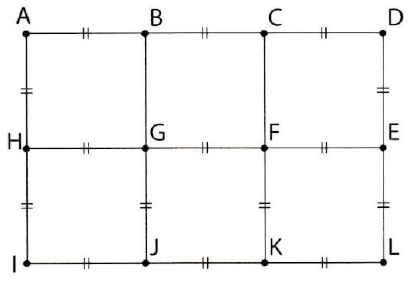
\includegraphics[width=.5\linewidth]{transformation-du-plan/img/ex02.png}
    \end{center}
    \begin{tasks}
        \task L'image de A par la symétrie d'axe $BJ$ est \dotfill
        \task L'image de F par la symétrie de centre $G$ est \dotfill
        \task La translation qui applique $I$ sur $G$ applique $K$ sur \dotfill
        \task La symétrie d'axe $IC$ applique $K$ sur \dotfill
        \task La translation qui applique $G$ sur $B$ applique $K$ sur \dotfill
        \task La symétrie de centre \dotfill applique $J$ sur $D$.
    \end{tasks}
